\documentclass{article}

\usepackage{fullpage}
\usepackage{amsmath}
\usepackage{tikz}

\usepackage{fancyhdr}
\pagestyle{fancy}
\renewcommand{\headrulewidth}{0pt}
\cfoot{\sc Page \thepage\ of \pageref{end}}

\begin{document}

{\large \noindent{}University of Toronto at Scarborough\\
\textbf{CSC A67/MAT A67 - Discrete Mathematics, Fall 2015}}

\section*{\huge Exercise \#1: Counting/Arrangements}

{\large Due: September 19, 2015 at 11:59 p.m.\\
This assignment is worth 3\% of your final grade.}\\[1em]
\textbf{Warning:} Your electronic submission on MarkUs affirms that this exercise is your own work and no
one else's, and is in accordance with the University of Toronto Code of Behaviour on Academic Matters,
the Code of Student Conduct, and the guidelines for avoiding plagiarism in CSC A67/MAT A67.\\[1ex]
This exercise is due by 11:59 p.m. September 19. If you haven't finished by then, you may hand in your
exercise late with a penalty as specified in the course information sheet.\\[1ex]
\renewcommand{\labelenumi}{\arabic{enumi}.}
\renewcommand{\labelenumii}{(\alph{enumii})}
\begin{enumerate}
\item Ruth has the following set of refrigerator magnets: \{A, B, C, D, E, F, G\}\marginpar{[3]}
	\begin{enumerate}
	\item How many different three-letter strings can she form with these magnets?
	\item How many different three-letter strings can she form if the middle lettter must be a vowel?
	\end{enumerate}
\item The school board consists of three men and four women. When they hold a meeting, they sit in a row.\marginpar{[7]}
	\begin{enumerate}
	\item How many different seating arrangments are there?
	\item How many different ways can the row be arranged if no two women sit next to each other?
	\item How many ways are there to select a subcommittee of four board members?
	\item How many ways are there to select a subcommittee of four board members if the subcommittee must contain at least two women?
	\end{enumerate}
\item There are nine empty seats in a theatre, and five customers need to find places to sit. How many different ways can these five seat themselves?\marginpar{[2]}
\item How many solutions (using only non-negative integers) are there to the following equation?\marginpar{[2]}
	\begin{equation*}
	x_1+x_2+x_3+x_4+x_5+x_6+x_7=20
	\end{equation*}
\item The North South Line of the Singapore Mass Rapid Transit system has 25 stations. How many ways are there to divide this line into three segments, where each segment contains at least one station? (One possible such division is shown below.)\marginpar{[2]}\\[1em]
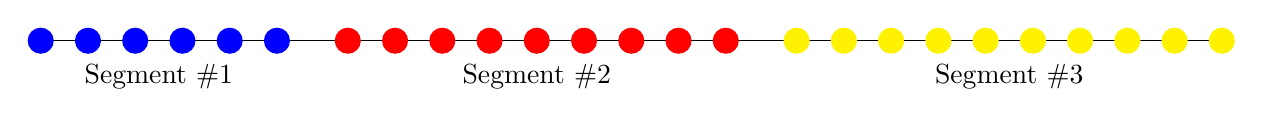
\begin{tikzpicture}[scale=0.6,station/.style={fill,circle,minimum size=2mm}]
\draw (0,0) node[station,fill=blue] {} \foreach \x in {1,...,5} { -- (\x,0) node[station,fill=blue] {}} -- (6.5,0);
\draw (6.5,0) node[station,fill=red] {} \foreach \x in {7.5,...,14.5} { -- (\x,0) node[station,fill=red] {}} -- (16,0);
\draw (16,0) node[station,fill=yellow] {} \foreach \x in {17,...,25} { -- (\x,0) node[station,fill=yellow] {}};
\draw (2.5,-.75) node {Segment \#1};
\draw (10.5,-.75) node {Segment \#2};
\draw (20.5,-.75) node {Segment \#3};
\end{tikzpicture}
\item If you are making a salad, and you must choose\marginpar{[2]}
	\begin{itemize}
	\item 1 of 2 dressings,
	\item at least 1 of 3 kinds of lettuce, and
	\item up to 4 other ingredients (tomatoes, cucumbers, etc.),
	\end{itemize}
how many different salad combinations can you make?
\end{enumerate}
\hrulefill\\
\noindent[Total: 18 marks]\label{end}

\end{document}